\documentclass[margin = 10pt]{standalone}
\usepackage{tikz}
\usepackage{pgfplots} 
\pgfplotsset{compat = 1.16}

\begin{document}
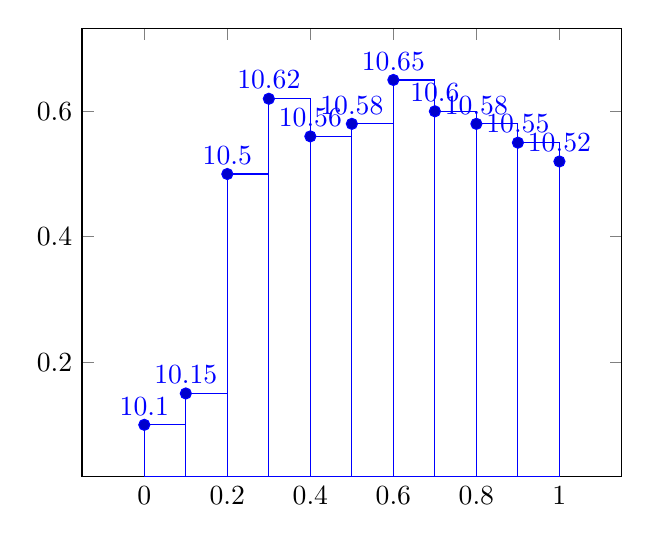
\begin{tikzpicture}
\begin{axis}[enlargelimits=0.15,]
\addplot+ [
    % ybar,
    ybar interval=0.1,
    bar width=7pt,nodes near coords,
    nodes near coords align={vertical},
    % 对meta 的y值进行运算
    point meta = y +10,
    ] coordinates {
        (0,0.1) (0.1,0.15) (0.2,0.5) (0.3,0.62)
        (0.4,0.56) (0.5,0.58) (0.6,0.65) (0.7,0.6)
        (0.8,0.58) (0.9,0.55) (1,0.52)
    };
\end{axis}
\end{tikzpicture}
\end{document}
